\chapter{Sequence prediction for running cases}
\label{chap:taking-inspiration}
While a number of works have demonstrated the applicability of LSTM neural networks to Predictive Process Monitoring, most have left out a perspective on the sequence prediction problem from Natural Language Processing (NLP). In this chapter we outline how we take inspiration from sequence prediction in NLP, and thus add to improvement area 3 from \autoref{sec:intro:contribution}.

We establish the connection between processes and sequences by connecting their definitions in \autoref{sec:contrib:case-sequence-understanding}. This provides the underpinning for introducing two NLP-inspired approaches for predicting the next activity in a case. These are presented in \autoref{sec:contrib:sp2-inspiration} and \autoref{sec:contrib:pfs-inspiration}.

\section{Understanding a trace as a sequence}\label{sec:contrib:case-sequence-understanding}
The definition for sequences presented in \autoref{sec:background:sequence-prediction} and the definition of traces in \autoref{sec:log-structure} will be connected in this section to make it clear how events can be understood as itemsets.

Both a trace $\#_{trace}(c)$ from a case $c$ and a sequence $seq$ are already defined in a very similar manner:
\begin{equation*}
\begin{split}
seq           &=  \langle s_1,s_2\cdots s_l \rangle\ |\ \forall\ 0 \leq j \leq l: s_j \subseteq \mathscr{I}\\
\#_{trace}(c) &= \langle e_1, e_2, e_3 \dots, e_n \rangle
\end{split}
\end{equation*}

Any itemset consists of items $s = (i_1, i_2 \cdots i_n)$ with $i \in \mathscr{I}$. Events are made up of attributes that are accessed via the $\#$ operator.
In a first step, attributes are defined as items, so that any possible value from any attribute can be understood as an item:

$$\mathscr{I} = \{\#_{a}(e)\ |\ c \in L\wedge e \in \#_{trace}(c) \wedge a \in attrs(e)\}$$

In a second step, a schema is applied to the itemsets. Without it, the itemset that should represent an event could consist e.g. only out of timestamps, as $s \subseteq \mathscr{I}$ does not place any restrictions on the content of $s$.
The schema also provides the tabular format required for machine learning applications, and is introduced as a direct mapping from event $e$ to itemset $s$:

$$ s = (i_1, i_2 \cdots i_n)\ |\ i_i = \#_{attrs(e)[i]}(e) $$

The definition places each item on a specific place in the itemset, depending on the index in the attribute list $attr(e)$. Still, the original condition $s \subseteq \mathscr{I}$ hold true, and now permits sequence prediction on traces.

\section{Adapting a competition submission}\label{sec:contrib:sp2-inspiration}
Shibata et al.'s bipartite network architecture has shown outstanding performance in the SPiCe competition~\cite{web:spice}. Under the assumption that a case exhibits properties similar to sentences, we adapt it for use in the business process domain.

\begin{figure}[!htb]
    \centering
    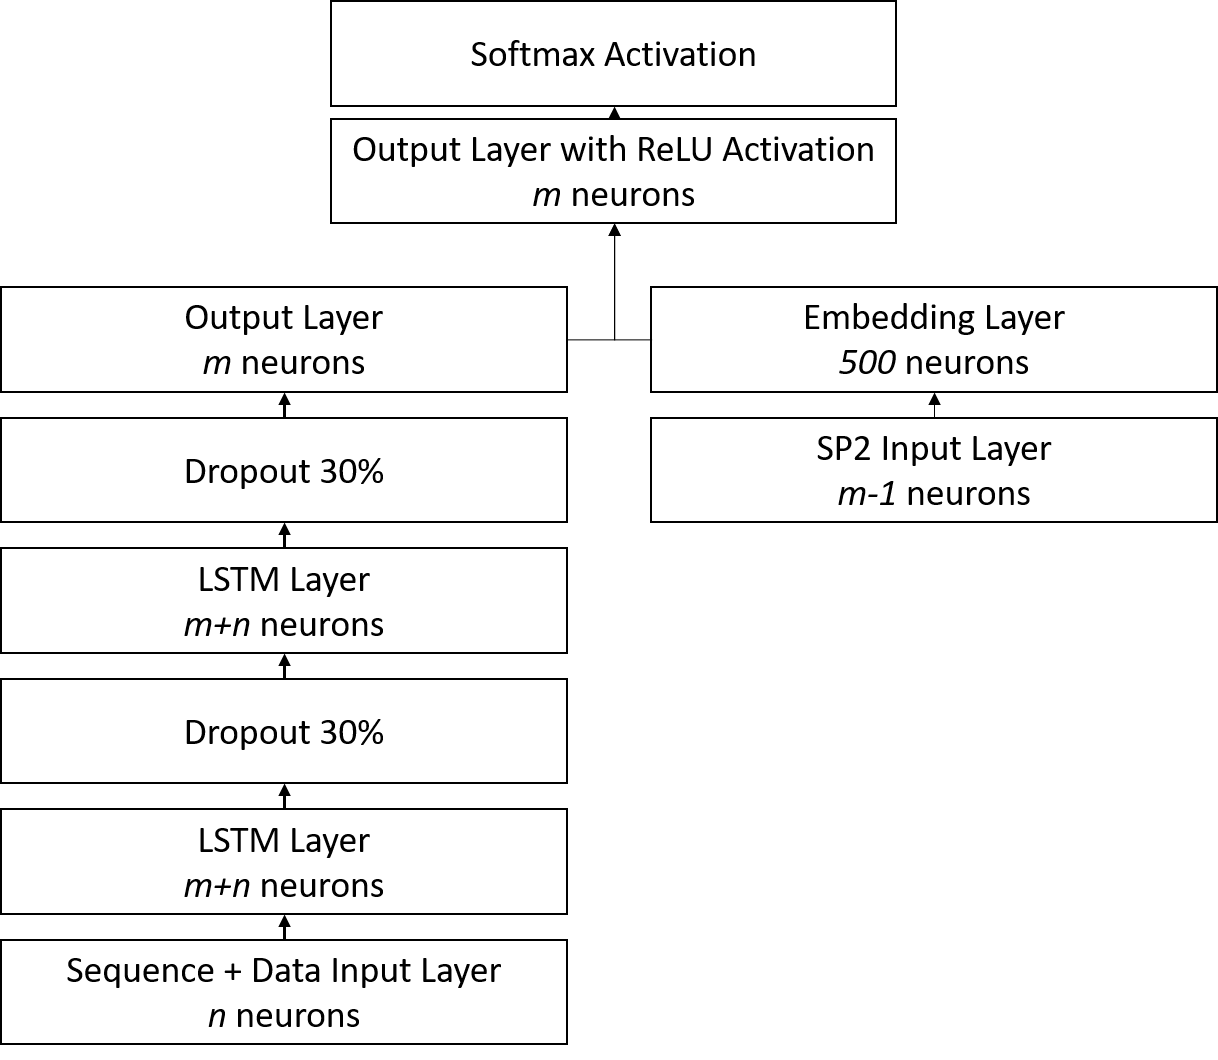
\includegraphics[width=0.8\textwidth]{gfx/sp2-network-architecture.png}
    \caption{The SP2 network architecture}
    \label{fig:sp2-architecture}
\end{figure}

\autoref{fig:sp2-architecture} displays the adapted network architecture from Shibata et al., and we shall describe the changes we made in the following.

The Embedding layers were completely removed. Above the SP-2 feature input layer, the embedding layer was replaced with a fully-connected layer. The reason for the removal is as follows: Shibata et al. predicted the next word in a sentence based on the preceding words, and as such, the itemsets that they used consisted of a single item: a word~\cite{shibata2016bipartite}. We aim to predict the next activity based on the preceding events, and as shown in the previous section, the event-itemsets consist of multiple items which represent different attributes.
Embedding layers require dictionary-encoded input of a single item, which is a problem when multiple items belong together~\cite{goldberg2014word2vec}. An alternative to the removal would have been the concatenation of the outputs of one Embedding layer per attribute type. We decided against this due to the relatively small amount of available training data and the increased computational overhead.

The model uses $n$ units on the first input layer, denoting the dimensionality of the input vector with its encoded activity name, timestamps and other event attributes. It puts out the next activity in one-hot encoded form through $m$ units, thus modelling the task as a multi-classification problem.

In contrast to Evermann et al. and Shibata et al., the number of units $m+n$ in the hidden layers is a function of the input unit count and the output unit count. This follows general advice not to introduce bottlenecks in the hidden layers by using fewer units than required in the output layer~\cite{web:techniques-in-convnets,szegedy2016rethinking}. Furthermore, dropout layers have been introduced to prevent overfitting.

The SP-2 features are to be engineered based on the activity names, as the name of the next activity is also the prediction target. Shibata et al. also encoded the history of the prediction target in their implementation~\cite{shibata2016bipartite}. The SP-2 features are fed in higher up on the right side of the tree, passing through a ReLU-activated, fully-connected layer, before concatenation with the LSTM output. Finally, the concatenated vectors are processed by fully-connected layers, with the commonly used Softmax activation function producing the classification.

\section{Encoding subsequence occurrence}
\label{sec:contrib:pfs-inspiration}
Klinkmüller et al. compared different feature representations and found that sub-trace occurence features can help models cover a broader variety of relationships~\cite{klinkmuller2018reliablemonitoring}. While they found this to be true for random forests, we want to investigate the applicability of such features for LSTM neural networks since we established the similarity of traces and sequences. While the results from Francescomarino et al. are discouraging~\cite{francescomarino2017}, another network architecture could make a difference.

Since SP-2 features already encode history and subsequence encodings do the same on a higher level of abstraction, we take the SP2 model architecture and inject different features in place of the SP-2 features. Said features and the corresponding architecture will henceforth be referred to as PFS, as illustrated in \autoref{fig:pfs-architecture}. The acronym PFS originates from the word PrefixSpan, which is the name of the algorithm used in \autoref{chap:evaluation} to mine the subsequences. Both PFS and SP2 models will be evaluated in \autoref{chap:evaluation}.

\begin{figure}[ht]
    \centering
    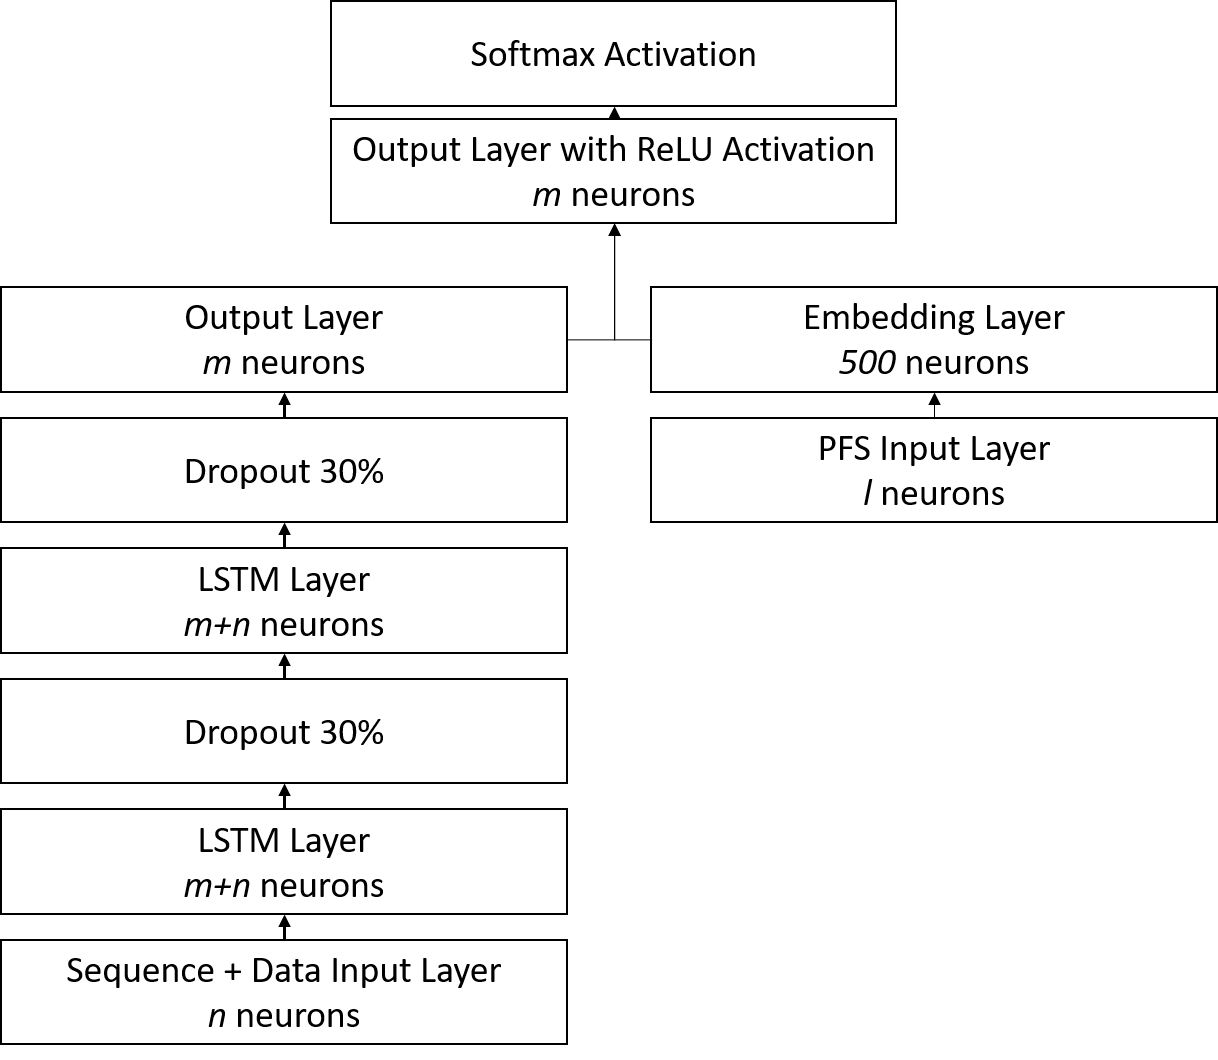
\includegraphics[width=0.8\textwidth]{gfx/pfs-network-architecture.png}
    \caption{The PFS network architecture}
    \label{fig:pfs-architecture}
\end{figure}
